\tikzset{every picture/.style={line width=0.75pt}} %set default line width to 0.75pt        

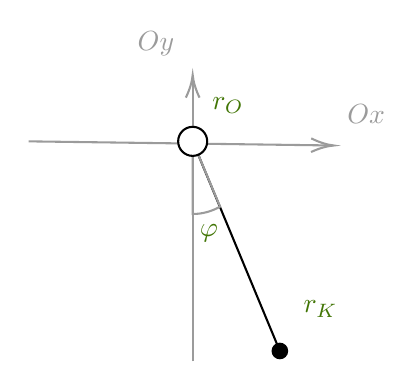
\begin{tikzpicture}[x=0.75pt,y=0.75pt,yscale=-1,xscale=1]
	%uncomment if require: \path (0,300); %set diagram left start at 0, and has height of 300
	
	%Straight Lines [id:da1514141660071826] 
	\draw [color={rgb, 255:red, 155; green, 155; blue, 155 }  ,draw opacity=1 ]   (171,175) -- (171,39) ;
	\draw [shift={(171,37)}, rotate = 90] [color={rgb, 255:red, 155; green, 155; blue, 155 }  ,draw opacity=1 ][line width=0.75]    (10.93,-3.29) .. controls (6.95,-1.4) and (3.31,-0.3) .. (0,0) .. controls (3.31,0.3) and (6.95,1.4) .. (10.93,3.29)   ;
	%Straight Lines [id:da8867696028247825] 
	\draw [color={rgb, 255:red, 155; green, 155; blue, 155 }  ,draw opacity=1 ]   (92,69) -- (237,70.97) ;
	\draw [shift={(239,71)}, rotate = 180.78] [color={rgb, 255:red, 155; green, 155; blue, 155 }  ,draw opacity=1 ][line width=0.75]    (10.93,-3.29) .. controls (6.95,-1.4) and (3.31,-0.3) .. (0,0) .. controls (3.31,0.3) and (6.95,1.4) .. (10.93,3.29)   ;
	%Straight Lines [id:da86988252841081] 
	\draw    (171,69) -- (213,170) ;
	%Shape: Circle [id:dp42453397326631825] 
	\draw  [fill={rgb, 255:red, 0; green, 0; blue, 0 }  ,fill opacity=1 ] (209.5,170) .. controls (209.5,168.07) and (211.07,166.5) .. (213,166.5) .. controls (214.93,166.5) and (216.5,168.07) .. (216.5,170) .. controls (216.5,171.93) and (214.93,173.5) .. (213,173.5) .. controls (211.07,173.5) and (209.5,171.93) .. (209.5,170) -- cycle ;
	%Shape: Pie [id:dp2450860928862184] 
	\draw  [color={rgb, 255:red, 155; green, 155; blue, 155 }  ,draw opacity=1 ] (184.19,100.45) .. controls (180.21,102.72) and (175.73,104) .. (171,104) -- (171,69) -- cycle ;
	%Shape: Circle [id:dp7741237432120269] 
	\draw  [fill={rgb, 255:red, 255; green, 255; blue, 255 }  ,fill opacity=1 ] (164,69) .. controls (164,65.13) and (167.13,62) .. (171,62) .. controls (174.87,62) and (178,65.13) .. (178,69) .. controls (178,72.87) and (174.87,76) .. (171,76) .. controls (167.13,76) and (164,72.87) .. (164,69) -- cycle ;
	
	% Text Node
	\draw (244,49.73) node [anchor=north west][inner sep=0.75pt]  [color={rgb, 255:red, 155; green, 155; blue, 155 }  ,opacity=1 ]  {$Ox$};
	% Text Node
	\draw (143,14.73) node [anchor=north west][inner sep=0.75pt]  [color={rgb, 255:red, 155; green, 155; blue, 155 }  ,opacity=1 ]  {$Oy$};
	% Text Node
	\draw (223,144.4) node [anchor=north west][inner sep=0.75pt]  [color={rgb, 255:red, 65; green, 117; blue, 5 }  ,opacity=1 ]  {$\bo{r}_{K}$};
	% Text Node
	\draw (179,46.4) node [anchor=north west][inner sep=0.75pt]  [color={rgb, 255:red, 65; green, 117; blue, 5 }  ,opacity=1 ]  {$\bo{r}_{O}$};
	% Text Node
	\draw (173,107.4) node [anchor=north west][inner sep=0.75pt]  [color={rgb, 255:red, 65; green, 117; blue, 5 }  ,opacity=1 ]  {$\varphi $};
	
	
\end{tikzpicture}
